\begin{figure*}[t]
    \centering
    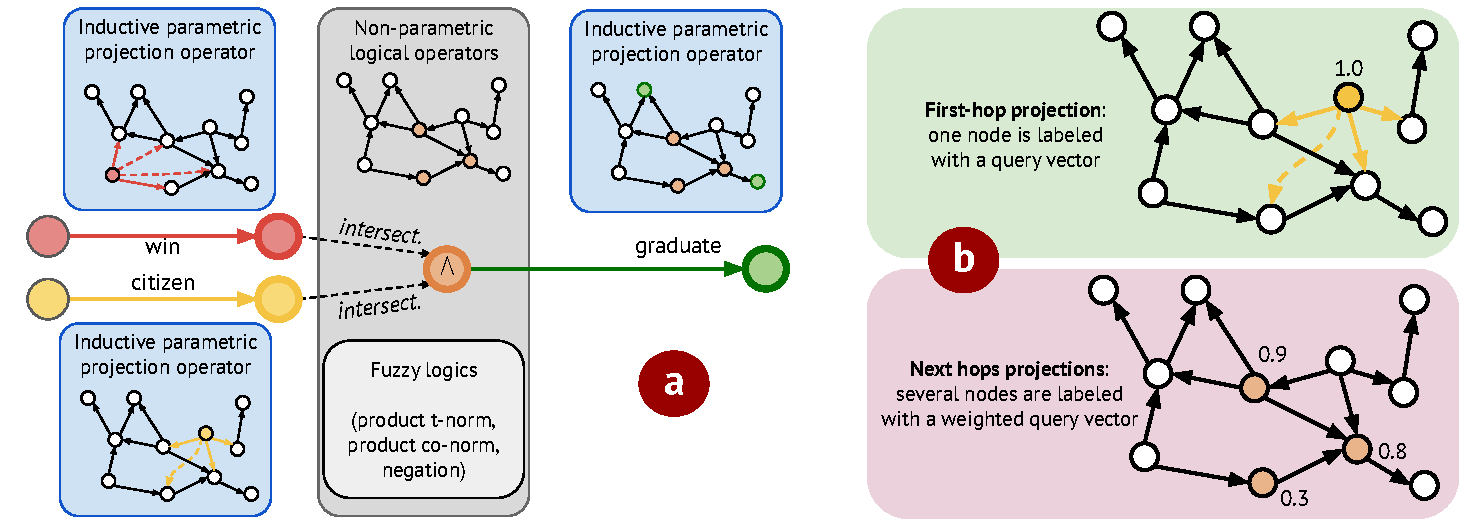
\includegraphics[width=\linewidth]{figs/Fig2v2.pdf}
    \vskip -0.1 in
    \caption{\textbf{(a)} Example of \emph{ip} query answering with \method: the inductive parametric projection operator (\Cref{subsec:ultra_proj}) executes relation projections on any graph and returns a scalar score for each entity; the scores are aggregated by non-parametric logical operators (\Cref{subsec:logic_ops}) implemented with fuzzy logics. Intermediate scores are used for weighted initializion of relation projections on the next hop. \textbf{(b)} The multi-source propagation issue with a pre-trained link predictor for relation projection: pre-training on  \emph{1p} link prediction is done in the single-source labeling mode (top) where only one query node is labeled with a non-zero vector; complex queries at later intermediate hops might have several plausible sources with non-zero initial weights %from intermediate results 
    (bottom) where a pre-trained operator fails. }
    \label{fig:ultraquery}
    \vskip -0.15 in
\end{figure*}

\section{Method}
\label{sec:method}

We aim at designing a single foundation model for \clqa on any KG in the zero-shot fashion, \ie, without training on a target graph.
In the \clqa literature~\citep{gqe,q2b,betae,cqd,gnn_qe}, it is common to break down query execution into a \emph{relation projection} to traverse graph edges and predict missing links, and \emph{logical operators} that model conjunction, disjunction, and union.
The main challenge boils down to designing inductive projection and logical operators suitable for any % unseen
entity and relation vocabulary.

\subsection{Inductive Relation Projection}
\label{subsec:ultra_proj}

The vast majority of \clqa methods are inherently transductive and implement relation projections as functions over entity and relation embeddings fixed to a certain KG vocabulary, \eg, with scoring functions from KG completion methods~\citep{gqe,cqd,qto}, geometric functions~\citep{q2b,cone}, or pure neural methods~\citep{mlpmix,lmpnn}.
The only method inductive to new entities~\citep{gnn_qe} learns relation embeddings and uses those as a labeling trick (\Cref{sec:prelim}) for a GNN that implements the projection operator.

As fixed relation embeddings do not transfer to new KGs with new relations, 
%in \method, 
we adapt \ultra~\citep{ultra}, an inductive approach that builds relation representations dynamically using the invariance of \emph{relation interactions}, as the backbone of the relation projection operator thanks to its good zero-shot performance on simple KG completion tasks across a variety of graphs.
\ultra leverages theoretical findings in multi-relational link prediction~\citep{rwl,rwl2} and learns relation representations from a \emph{meta-graph} of relation interactions\footnote{The meta-graph can be efficiently obtained from any KG.}.
The meta-graph includes four learnable edge types or meta-relations (\emph{head-to-tail}, \emph{tail-to-head}, \emph{head-to-head}, \emph{tail-to-tail}) which are independent from KG's relation vocabulary and therefore transfer across any graph.
Practically, given a graph $\gG$ and projection query $(h, r, ?)$, \ultra employs labeling trick GNNs on two levels.
First, it builds a meta-graph $\gG_r$ of relation interactions (a graph of relations where each node is a unique edge type in $\gG$) and applies a labeling trick to initialize the query node $r$. 
Note that $|\gR| \ll |\gE|$, the number of unique relations is much smaller than number of entities in any KG, so processing this graph of relations introduces a rather marginal computational overhead.
Running a message passing GNN over $\gG_r$ results in \emph{conditional relation representation} which are used as initial edge type features in the second, entity-level GNN.
There, a starting node $h$ is initialized with a query vector from the obtained relation representations and running another GNN over the entity graph (with a final sigmoid readout) returns a scalar score in $[0, 1]$ representing a probability of each node to be a tail of a query $(h,r,?)$.

The only learnable parameters in \ultra are four meta-relations for the graph of relations and GNN weights. The four meta-relations represent structural patterns 
%like “a tail of and edge with relation X is the head of another edge with relation Y” 
and can be mined from any multi-relational KG independent of their entity and relation vocabulary. 
GNN weights are optimized during pre-training. Since the model does not rely on any KG-specific entity or relation vocabulary, a single pre-trained \ultra model can be used as a zero-shot relation projection operator on any KG. \autoref{fig:ultraquery}(a) illustrates the \emph{intersection-projection} query execution process where each projection step is tackled by the same inductive projection operator with initialization depending on the start anchor node or intermediate variables.

\textbf{The multi-source propagation issue.}
% \zz{We haven't introduced any idea of pre-trained KG models for relation projection so far.}
While it is tempting to leverage \ultra pre-trained on multiple KG datasets for relation projection, there is a substantial distribution shift (\autoref{fig:ultraquery}(b)) between KG completion and \clqa. Specifically, KG completion is a special case of relation projection where the input always contains a single node.
% The intermediate steps, however, present a conceptual challenge (\autoref{fig:ultraquery}(b)), that is, 
% a relation projection operator pre-trained on KG completion (equivalently, on \emph{1p} queries) is tailored for the \emph{single source, multiple tails} message passing when only one query node is initialized with a non-zero vector. 
% On the other hand,
By comparison, in multi-hop complex queries, several likely nodes might have high intermediate scores and will be labeled with non-zero vectors leading to the \emph{multiple sources} %, multiple tails}
propagation mode where a pre-trained operator is likely to fail.
To alleviate the issue, we experimentally study two strategies: (1) short fine-tuning  of the pre-trained projection operator on complex queries (used in the main \method model), or (2) use the frozen pre-trained operator and threshold intermediate scores setting all scores below $0 < k < 1$ to zero (denoted as \methodlp). The insight is to limit the propagation to one or a few source nodes, thereby reducing the discrepancy between training and test distributions.

%\ultra demonstrates generalization to dozens of unseen KGs in the zero-shot fashion outperforming many tailored inductive baselines.

% \zz{May retell Vapnik's definition of transductive and inductive inference here.
% \url{https://axon.cs.byu.edu/~martinez/classes/778/Papers/transductive.pdf}}

% \zz{
% \begin{enumerate}
%     \item (4.1) Definition of inductive and transductive models. May adapt from Vapnik's definition. Generally the idea is that transductive setting assumes the test vocabulary is known beforehand (which is identical to the training one in the setup of KGs).
%     \item Our goal: develop an inductive model for CLQA.
%     \item Following existing works (GQE, Q2B, BetaE, CQD, GNN-QE, etc.), CLQA is often handled by decomposing the query into relation projection operation and logical operations (conjunction, disjunction, negation).
%     \item The challenge boils down to: how to design inductive relation projection operations, and inductive logical operations? We try to answer this question with designs from existing methods.
%     \item (4.2) Inductive relation projection: Discuss why GQE, Q2B, BetaE, CQD are not inductive. Discuss why GNN-QE is inductive for entity vocabularies, but not for relation vocabularies.
%     \item How can we make a relational GNN (i.e. the family of suitable GNNs for GNN-QE) inductive for relation vocabularies? The idea is to parameterize relation embeddings as a function of a meta graph describing the relations (cite Ultra).
% \end{enumerate}
% }

% \zz{The implication of this story: based on what we know about existing complex query methods (we know a lot in our survey), the simplest choice for an inductive model is to combine GNN projection, relation meta-graph and fuzzy logic operation. Try not to mention GNN-QE as a whole, but derive GNN projection and fuzzy logic operation separately.}
% \subsection{GNN-QE as Inductive Query Executor}
%\paragraph{Learning Relation Representations from a Meta Graph}
%\zz{Reviewers didn't know NBFNet when we wrote GNN-QE. I would not assume the reviewers know Ultra well. So try to retell the idea and cite the paper rather than refer to the method.}
% \subsection{\ultra as a Universal Relation Projection Module}


\subsection{Inductive Logical Operations}
\label{subsec:logic_ops}

%     \item (4.3) Inductive logical operations: Discuss why GQE, Q2B, BetaE are not inductive. Their operations are learned to fit a particular entity embedding space. The only inductive solution from existing method is the t-norms and t-conorms from CQD, GNN-QE, QTO.
%     \item (4.4) Training \& optimization tricks: e.g. thresholding. Or maybe we want to put them to implementation details?
Learnable logical operators parameterized by neural nets in many \clqa approaches~\cite{gqe,q2b,cone,mlpmix} fit a particular embedding space and are not transferable.
Instead, we resort to differentiable but non-parametric \emph{fuzzy logics}~\citep{vankrieken_fuzzy} that implement logical operators as algebraic operations (\emph{t-norms} for conjunction and \emph{t-conorms} for disjunction) in a bounded space $[0,1]$ and are used in several neuro-symbolic \clqa approaches~\citep{cqd, gnn_qe, cqda, qto, fit}. 
%In fuzzy logics, \emph{t-norms} correspond to soft conjunctions, \emph{t-conorms} to disjunctions, and negation is often implemented as $1-x$ for bounded
\method employs fuzzy logical operators over \emph{fuzzy sets} $\vx \in [0,1]^{|\gV|}$ as the relation projection operator assigns a scalar in range $[0,1]$ for each entity in a graph. 
The choice of a fuzzy logic is often a hyperparameter although \citet{vankrieken_fuzzy} show that the \emph{product logic} is the most stable. 
In product logic, given two fuzzy sets $\vx, \vy$, conjunction is element-wise multiplication $\vx \odot \vy$ and disjunction is $\vx + \vy - \vx \odot \vy$.
Negation is often implemented as $\mathbf{1}-\vx$ where $\mathbf{1}$ is the \emph{universe} vector of all ones.
For second- and later $i$-th hop projections, we obtain initial node states $\vh_v$ by weighting a query vector $\vr_i$ with their probability score $x_v$ from the fuzzy set of a previous step: $\vh_v = x_v \vr_i$.


\subsection{Training}
Following existing works~\citep{betae,gnn_qe}, \method is trained on complex queries to minimize the binary cross entropy loss
\begin{align}
%\resizebox{.88\columnwidth}{!}{
\hspace{-0.5em}\displaystyle{
        \gL = -\frac{1}{|\gA_{q}|}\sum_{a \in \gA_{q}}\log p(a|q) 
              -\frac{1}{|\gV\backslash\gA_{q}|}\sum_{a' \in \gV\backslash\gA_{q}}\log (1 - p(a'|q))}
              %}
    \label{eqn:loss}
\end{align}
where $\gA_{q}$ is the answer to the query $q$ and $p(a|q)$ is the probability of entity $a$ in the final output fuzzy set.
\methodlp uses a frozen checkpoint from KG completion and is not trained on complex logical queries.

% talk about the main challenge: single-source message propagation vs multi-source propagation in the later hops of query answering